\section{System Model}
\label{system model}

    % \subsection{Traffic model}
    % \begin{figure}[t]
    % \centering
    % 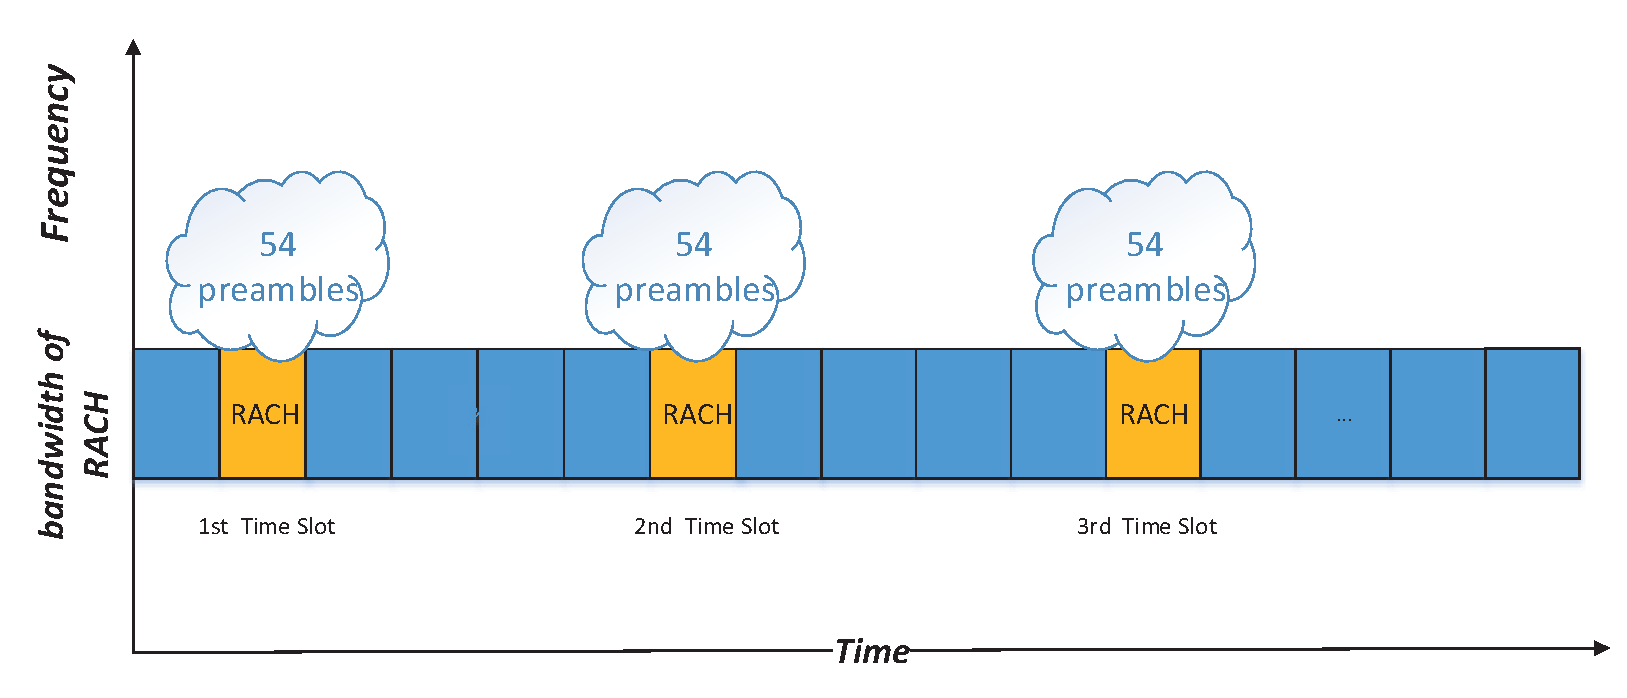
\includegraphics[width=5in]{fig_time_slot.eps}
    % \caption{Time slots of random access (1 slot = 1 ms) }
    % \label{fig time slot}
    % \end{figure}


    Consider that when an extreme scenario (e.g., power outage, earthquake) happens, MTC devices will try to reestablish synchronization with eNB in a short time period. In order to simulate the extreme scenario in which a large amount of MTC devices access network in a highly synchronized manner, we adopt traffic model 2 (Beta distribution) mentioned in~\cite{3GPP37.868} as arrival distribution and set the PRACH configuration to $6$, which means RACH will occur every $5 ms$ within 180 kHz. In our system model, we consider that there are total $N_{sys}$ MTC devices and then we define a time slot as an RACH slot so that the arrival period will be $2000$ time slots indexed by an nonnegative integer $j \ (j = 0, 1, 2, . . . , 2000)$ by reason of the $10$ seconds distribution period according to traffic model 2.
    \begin{eqnarray}
        p(t)=\frac{t^{\alpha-1 }(T-t)^{\beta -1}} {T^{\alpha + \beta -1} Beta(\alpha,\beta)},
    \end{eqnarray}
     where $Beta(\alpha,\beta)$ is the Beta function and $\alpha=3, \beta=4$.


    \begin{figure}[t]
    \centering
    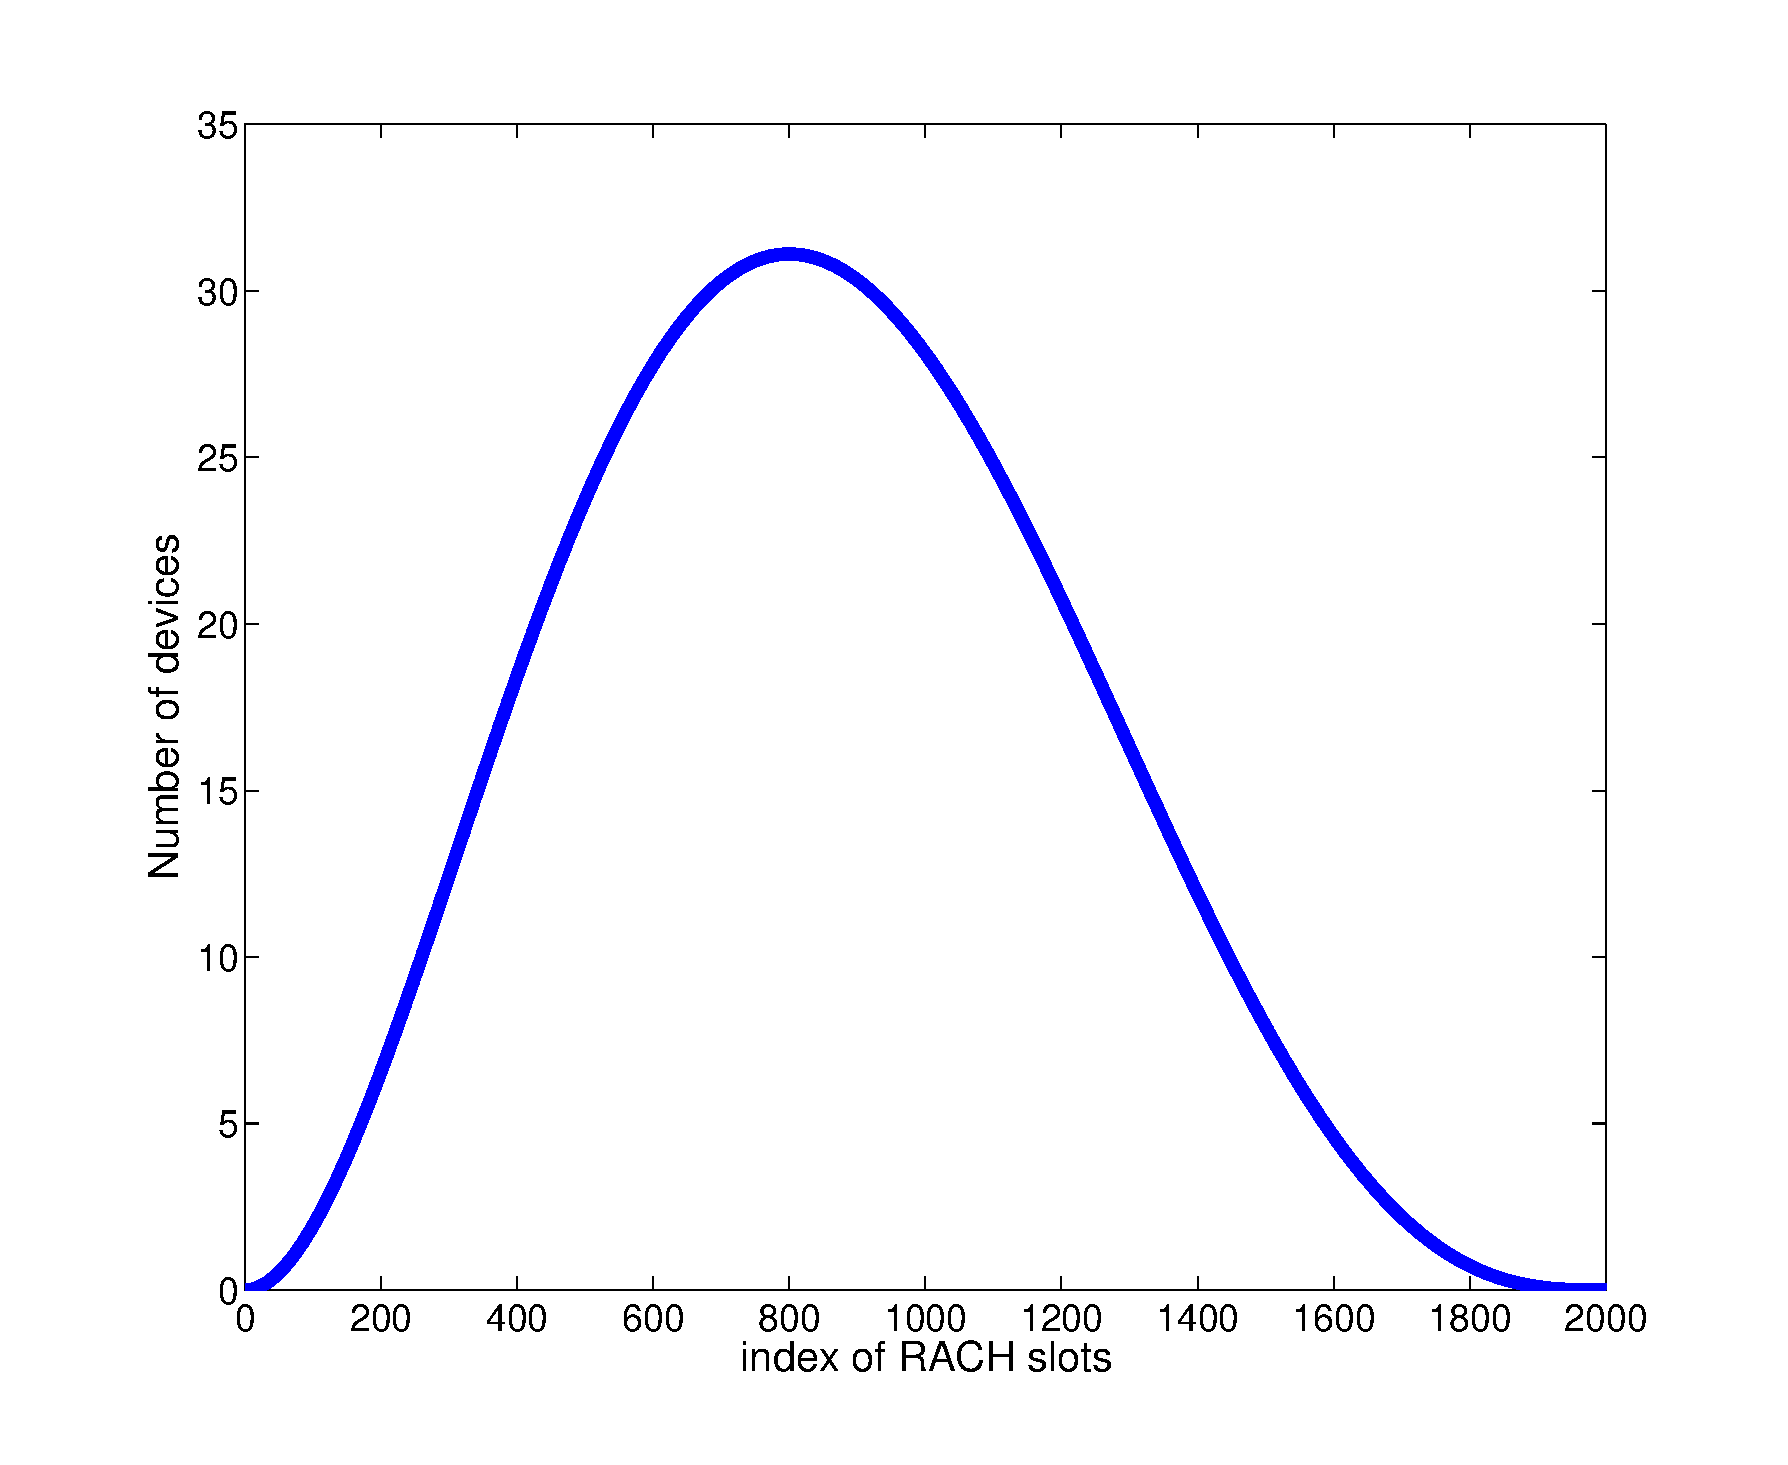
\includegraphics[width=3.8in]{fig_beta_distribution}
    \caption{Arrival period}
    \label{fig_beta_distribution}
    \end{figure}
     With the knowledge of above, equation $(1)$ is the probability that each MTC device will perform preamble transmissions at $t^{th}$ RACH slot during $T$ limited distribution of access attempts. As a result, the number of MTC devices $N^j$ that perform preamble transmissions at the $j^{th}$ RACH slot is shown in the following equation
    \begin{eqnarray}
      N^j=N_{sys}\int_{t_{j-1}}^{t_j}p(t)dt,\quad  j=1,2,...,2000,
    \end{eqnarray}
    where $t_j$ is the $j^{th}$ RACH slot. The arrival period calculated by equation $(2)$ is also in Fig.~\ref{fig_beta_distribution}.

    \subsection{Random Access Procedure}
    % \begin{figure}[t]
    % \centering
    % 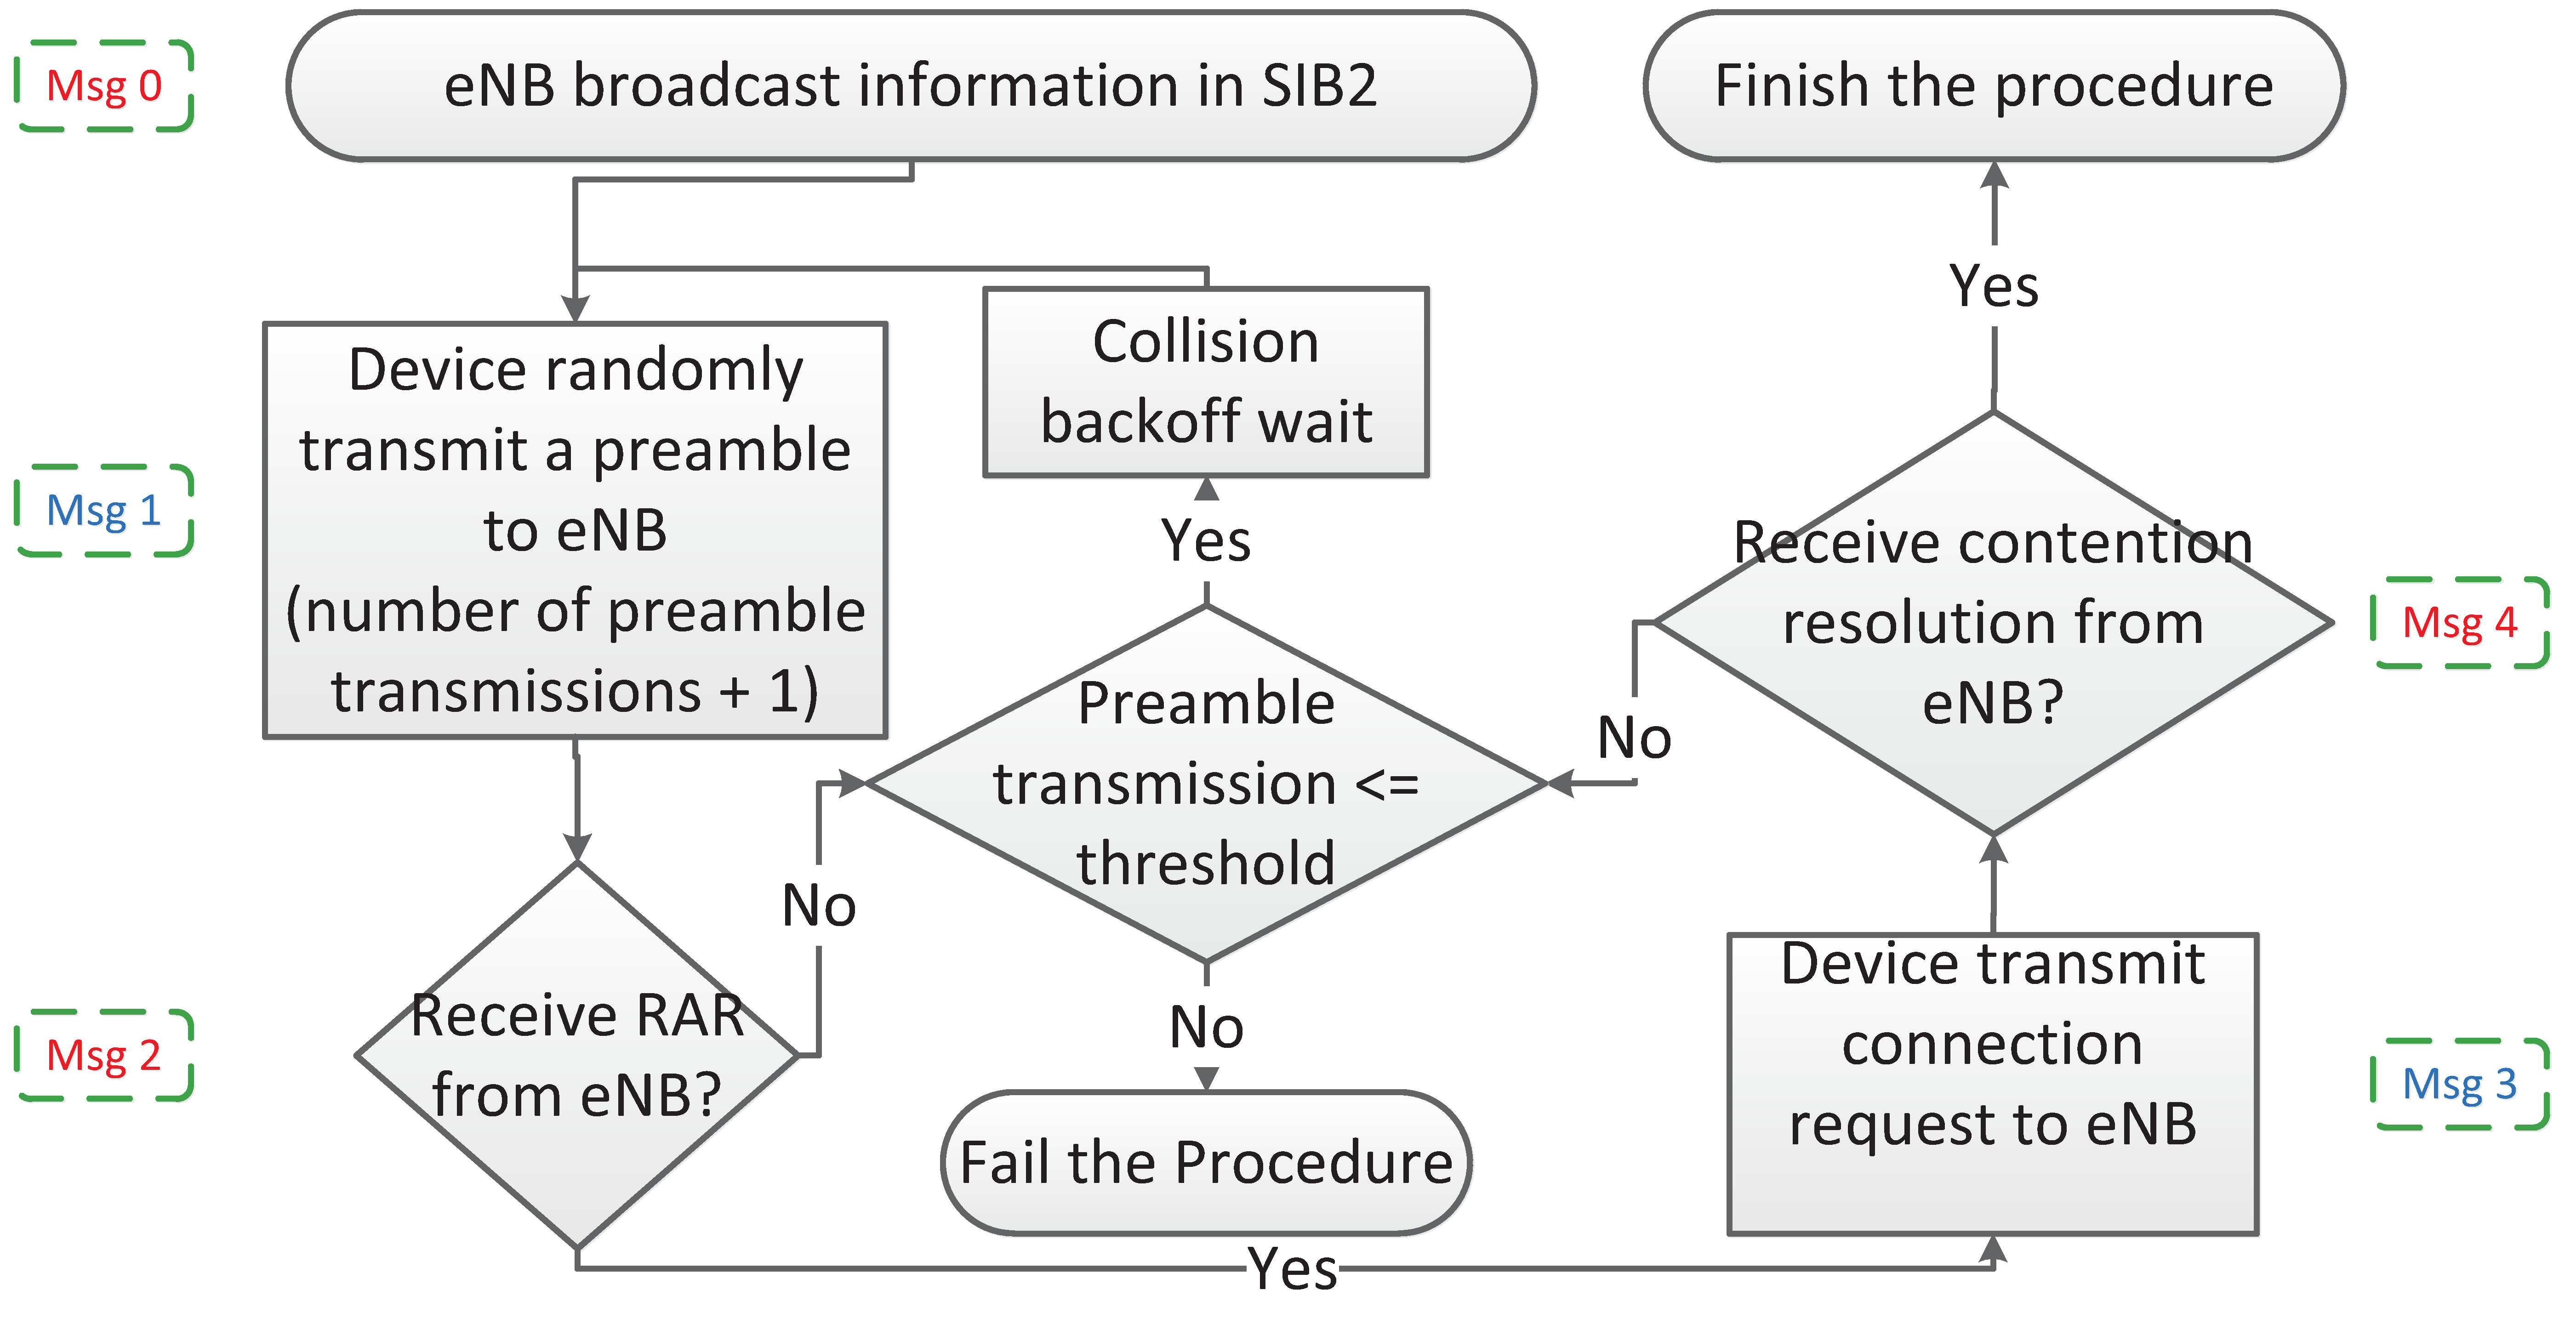
\includegraphics[width=5in]{fig_RA_flow_chart.eps}
    % \caption{Random access flow chart}
    % \label{fig_RA_flow_chart}
    % \end{figure}
    % Fig.~\ref{fig_RA_flow_chart} shows the flow chart of traditional random access procedure. Nevertheless, prior to performing random access, MTC devices will receive the information about random access procedure from system information block2 (SIB2) (e.g., available preambles $R$, backoff time) shown in Fig.~\ref{fig_broadcast}.
    % \begin{figure}[t]
    % \centering
    % 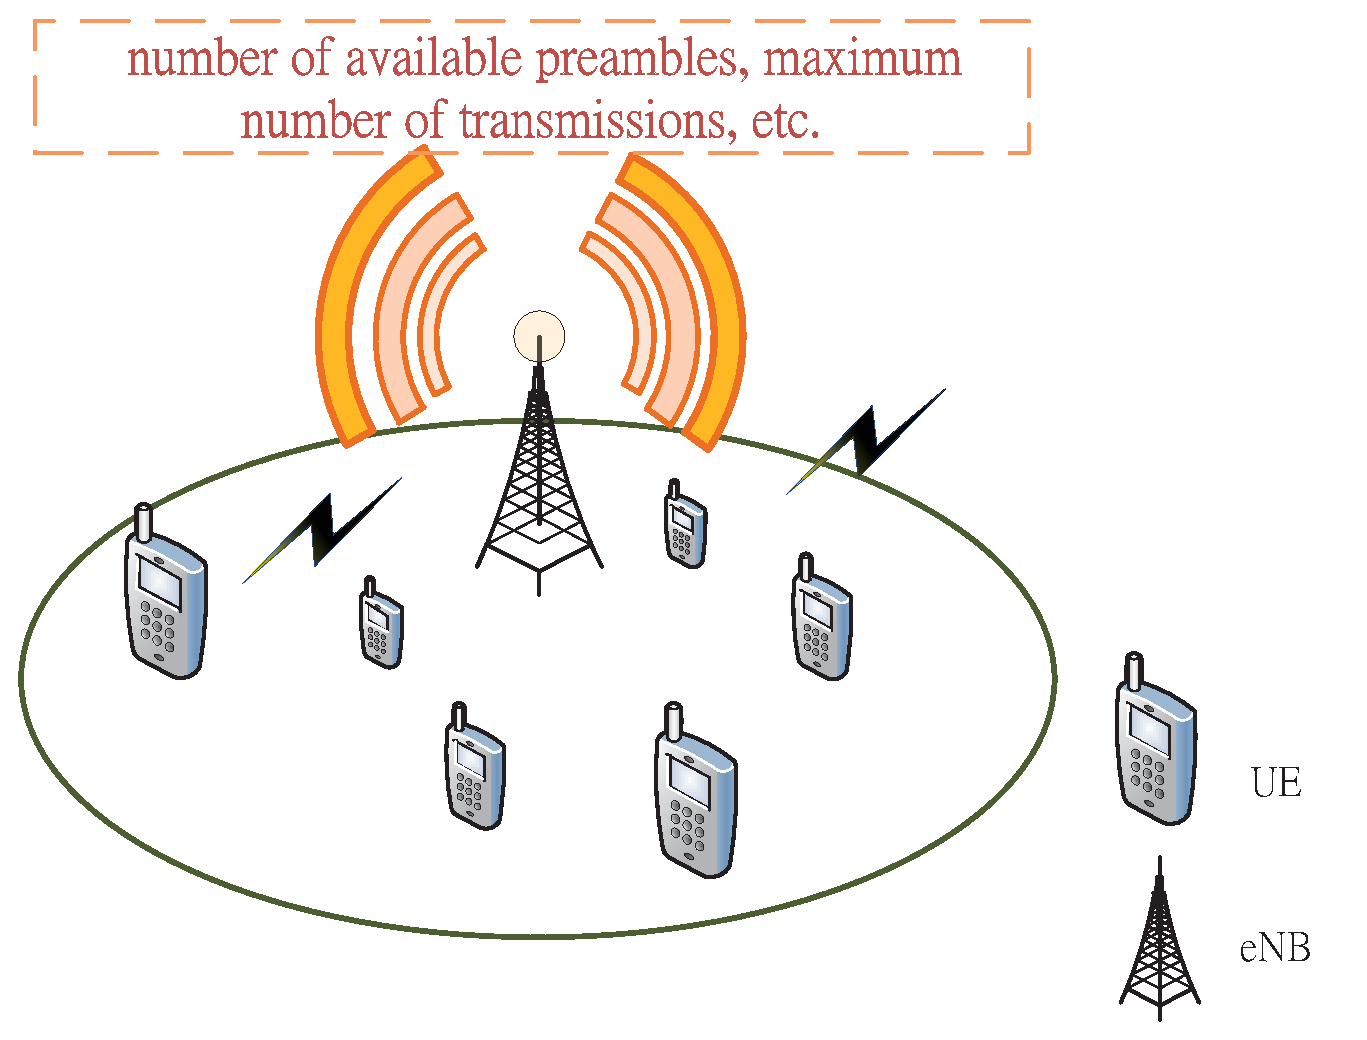
\includegraphics[width=5in]{fig_broadcast.eps}
    % \caption{Information of random access broadcasted by eNB}
    % \label{fig_broadcast}
    % \end{figure}
    After knowing the parameter of random access, each MTC device will randomly choose a preamble from the preamble pool, and the MTC device will increase the number of preamble transmissions by one and wait for RAR (Msg2). Upon receiving the Msg2 in the RAR window, the MTC device processes UL grant and Timing Alignment and prepare for sending the connection request (Msg3). If the MTC device fails to receive Msg2 in the RAR window due to the reason that eNB fails to detect the preamble from the device, it checks whether its number of preamble transmission is smaller or equal to the maximum number of preamble transmission. If it is, the MTC device retries to perform preamble transmission after waiting a uniform backoff time. If not, the MTC device is informed of random access procedure failure and it is not allowed to perform the procedure. Moreover, if the MTC device fails to receive contention resolution after sending connection request due to the collision of Msg3, it performs the same behavior of failing to receive RAR. We assume that once an UE successfully transmits the preamble chosen only by itself to eNB, and it will finish the RA procedure.
    In conclusion, eNB can get the number of collision preambles and success preambles, but it cannot get the total number of devices who perform the preamble transmission $N^j$ in an RACH slot $j$.

    \subsection{Access Class Barring Scheme}
    % \begin{figure}[t]
    % \centering
    % 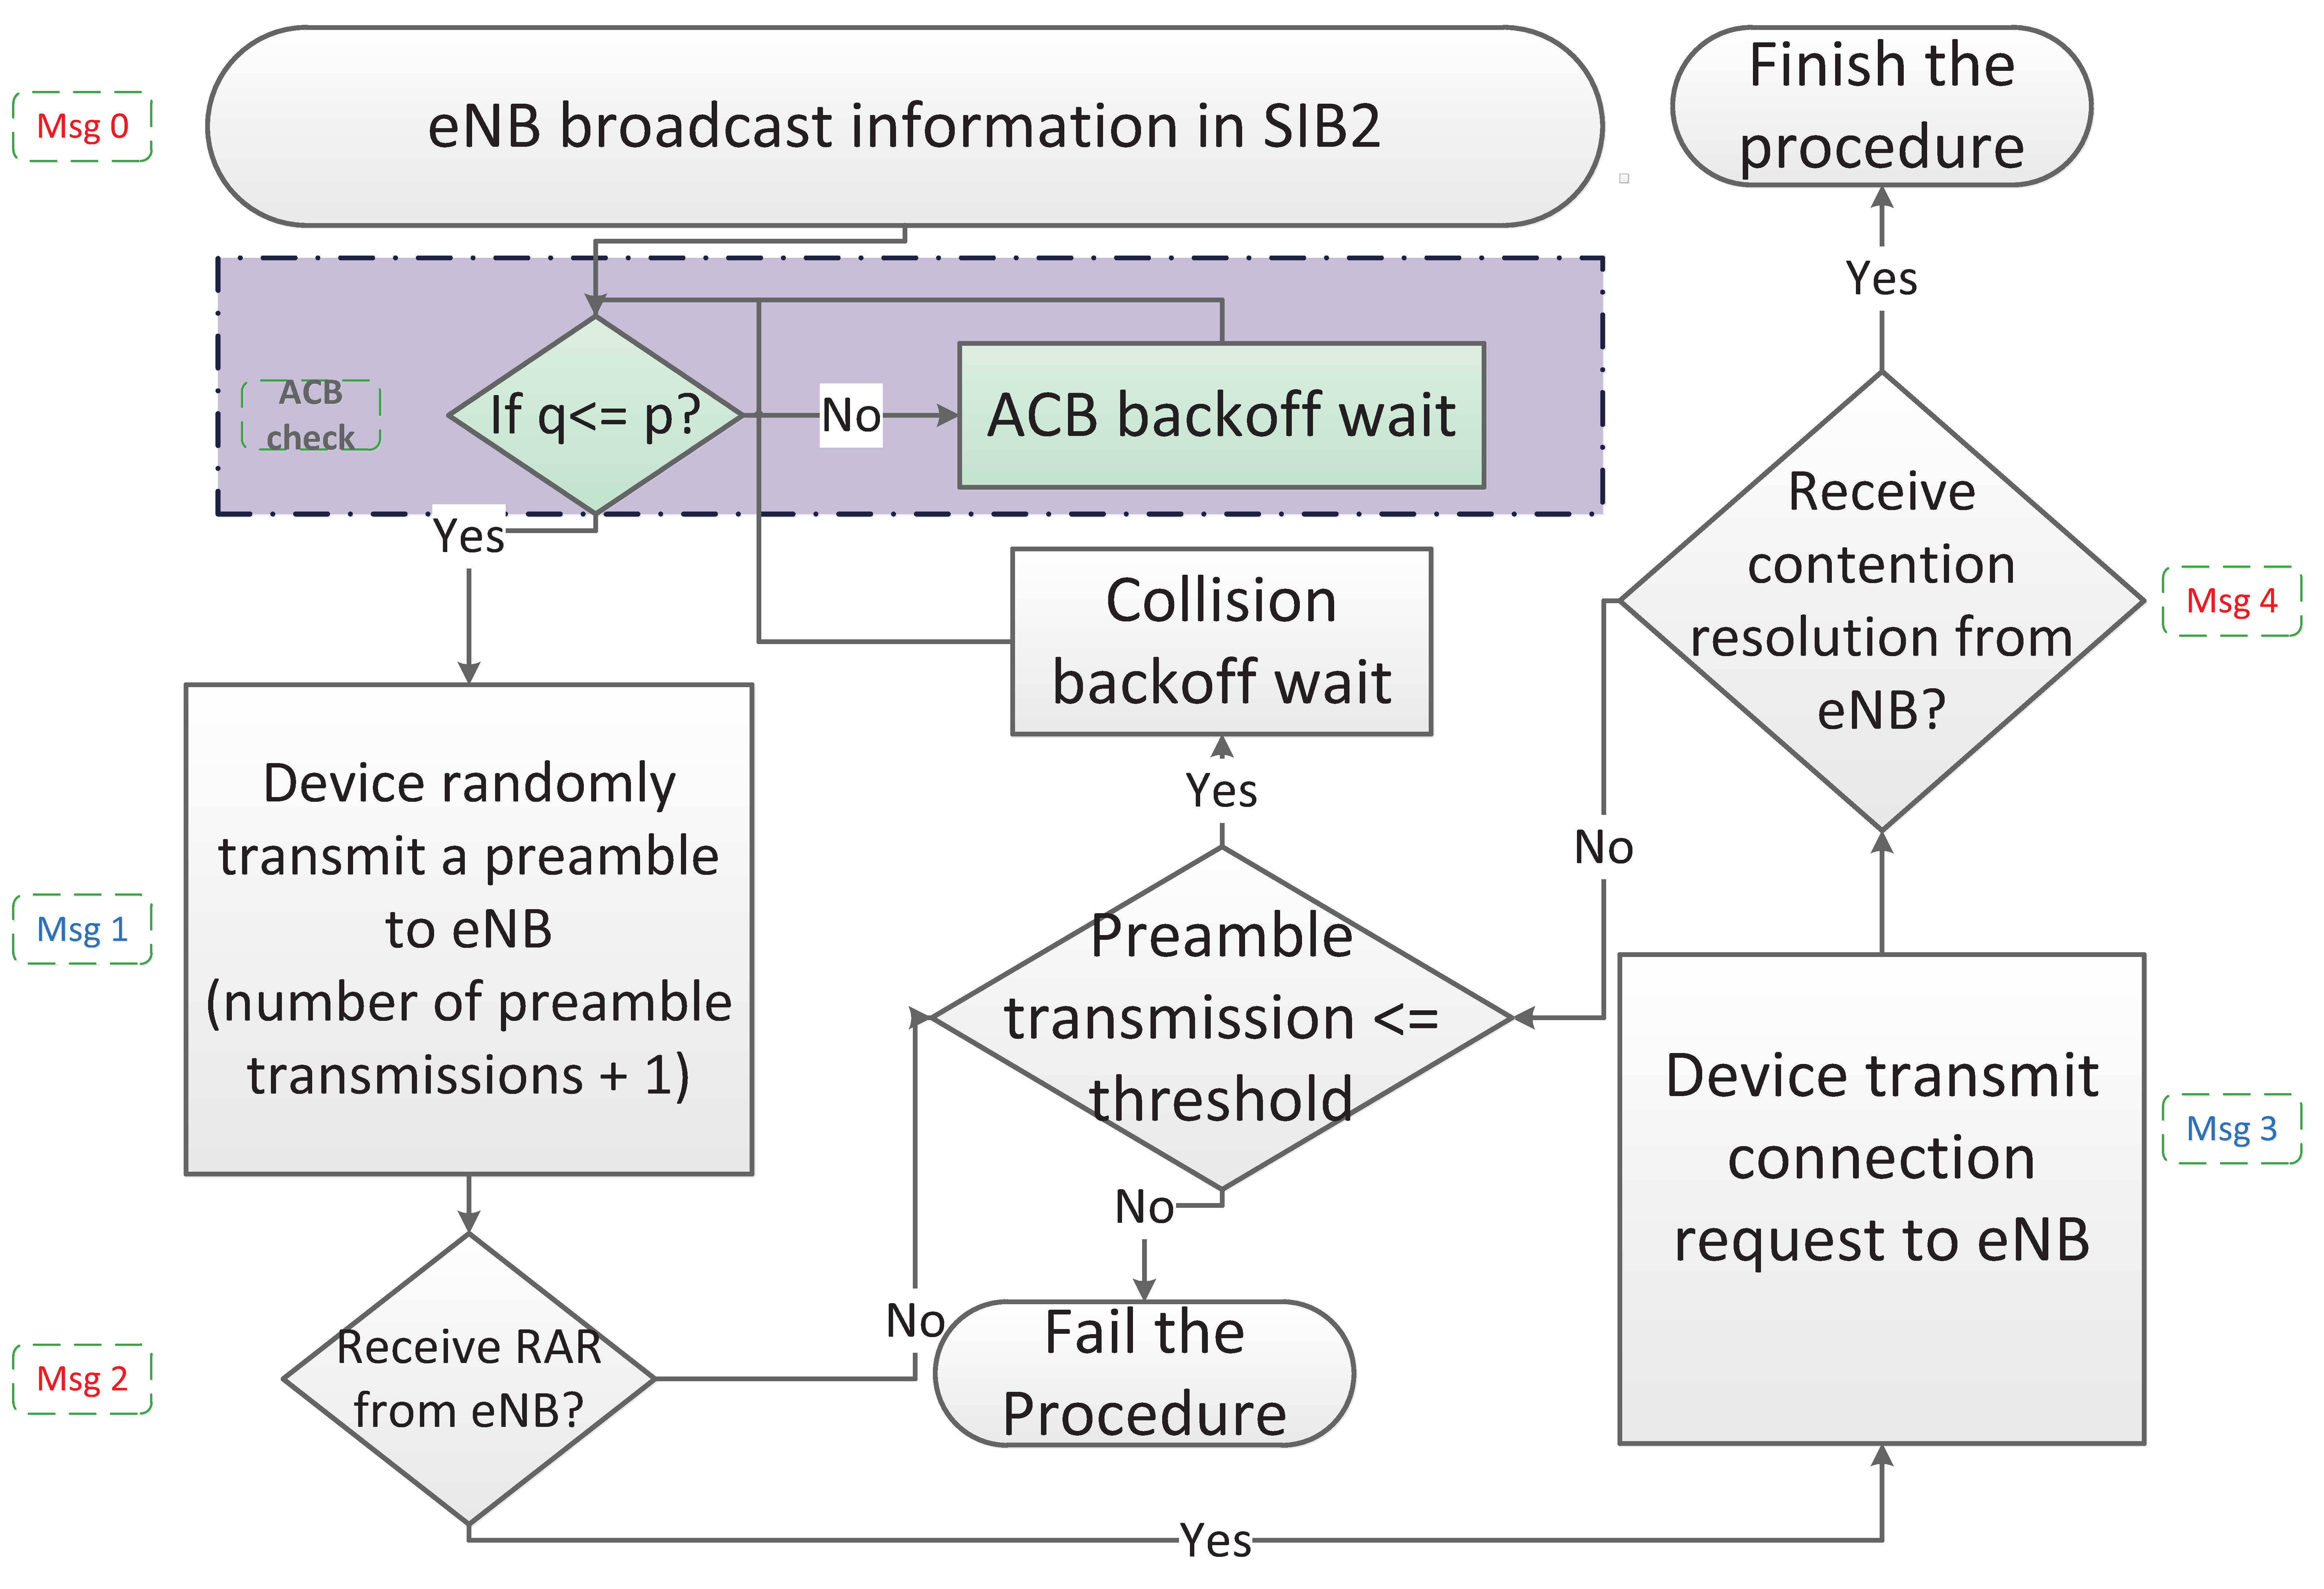
\includegraphics[width=5in]{fig_ACB_flow_chart.eps}
    % \caption{ACB flow chart}
    % \label{fig_ACB_flow_chart}
    % \end{figure}
    % Fig.~\ref{fig_ACB_flow_chart} shows the flow chart of ACB. 
    In ACB mechanism, the active MTC devices try to pass through the ACB factor $p$ broadcasted by eNB. Each MTC device draws a random value $q$ which between $0$ and $1$. If $q$ is less than $p$, we pronounce the devices pass through the ACB and it is allowed to perform random access procedure. Otherwise, it will be barred for a period of backoff time of ACB and repeat ACB scheme.

    \subsection{Performance Metric}
    The metric considered as an access success probability is defined as the probability to successfully complete the random access procedure within the maximum number of retransmissions~\cite{3GPP37.868}. The other metric we considered is the access delay defined as the RACH slots for each random access procedure between the first random access attempt and the completion of the random access procedure, for the successfully MTC devices.
